\documentclass[a4paper,10pt]{IEEEtran} \usepackage[margin=1.0in]{geometry} \usepackage{pdfpages} \usepackage{graphicx} 
\graphicspath{/graphics} \setlength{\parskip}{\baselineskip} \setlength\parindent{24pt}

\newcommand*\Title{WYSIWYG Approach to GUI for TensorFlow Deep Learning API}
\newcommand*\Date{October 2016}
\newcommand*\Author{Behnam Saeedi, Connor Sedwick, Collin Dorsett}
\newcommand*\GroupNumber{Group Number: 33}
\newcommand*\GroupName{Group Name: Visual Flow}
\title{WYSIWYG Approach to GUI for TensorFlow Deep Learning API}
\author{Behnam Saeedi, Connor Sedwick, Collin Dorsett}
\date{\today}

\begin{document}

	\begin{titlepage}
%	\includepdf[pages=1-,pagecommand={\thispagestyle{article}}]{myletter.pdf}
%		\maketitle
		\vspace*{\fill}
			\begin{center}
				\noindent \textbf{\Huge\Title} \\ 
				\large\Author \\ 
				\large\Date \\ 
				\large\GroupNumber \, \large\GroupName 
			\end{center}
			\noindent \textbf{Abstract} \\
			\indent 
			Software that allows individuals to visualize the step-by-step process of computer programming has greatly assisted aspiring programmers and experienced professionals.
	In the professional world, visualization software allows people in industry a tool to analyze data and develop a more concrete understanding of the architecture of a system. 
	Tools that aid individuals in programming software exist for both educational and commercial purposes, but there is a lack of visualization software targeted specifically at the subject of machine learning.
			TensorFlow is a machine learning API (Application Program Interface) developed by Google in order to provide an optimized machine learning toolset for developers.
			 This toolset is designed to be an all-in-one machine learning solution for users who do not have the time, technical skills or resources to produce their own methods.
			 Despite TensorFlow having useful applications and a rich manual it does not have an eloquent way to interact with visualization of the software for its users.
			 To address this issue we wish to develop a product that can display data between nodes in a computational graph and designing a network would be as easy as placing nodes and drawing connections between them.
			 This solution will take advantage of simple shapes to abstract basic programming concepts.
			 This system will represent the complext program as simple flowchart like diagrams to the user.
			 Another important aspect of our system is Runtime Tuning.
			 Runtime Tunning is manipulation of data and variables during the runtime of a program in order to help users in improving the performance of their solution.
			 Our proposed Graphical User Interface (GUI) will offer sets of features in order to make this task easier.
			 Our target audience is individuals with little to no experience with machine learning or computer programming who specialize in fields such as statistics, data analysis and mathematics.\\
		\vspace*{\fill}
	\end{titlepage}

	\noindent \textbf{Problem Definition}\\
	\indent TensorFlow, an API developed by Google is a Deep Learning developer tool that requires much technical knowledge to implement and run.
	 We need to develop a GUI (graphical user interface) that allows users the ability to access TensorFlow methods, use them to create a program and visualize its control flow.
	 We need to develop an interface that is easy to navigate while also providing useful feedback to the user if there is an error in their implementation.
	 It should be easy to install and support multi-layered program designs. It should also allow users to input different types of data (i.e. graphical data or text).
	 Furthermore, this software needs to support a simple drag, drop and connect functionality to enhance user experience.\\

	\noindent \textbf{Proposed Solution}\\
	\indent Our proposed solution is to use the Python scripting language to develop a software that grants developers the ability to graphically visualize the control flow of their program using a flowchart style design backed with TensorFlow API.
	 It will also track states of the program between methods during execution to aid monitoring and modifying run-time parameters.
	 Furthermore, this software will warn users if they are missing a specific node required in their program that is required for it to compile and run correctly.\\
	 \\The following is how we plan to model our solution:
	\begin{itemize}
		\item Display the build space in a graphical user interface. This display is called the Scene.
		\item Represent variables as blocks. These blocks contain data.
		\item Represent methods as blocks. These blocks can be rotated in order to help with readability. Furthermore, you can adjust the visual size of this block.
		\item Represent classes as blocks. Classes can contain multiple method and variable blocks and could be abstracted away.
		 when a class is abstracted, it is represented as a new block that hides its members.
		\item Represent layers as pages. Layers can contain multiple classes, however, each layer is independent of other layers. Layers could be disabled or enabled.
		\item Represent input and output arguments as circles on method blocks
		\item Represent channels as vectors. A channel is a connection between an input and an output that describes how data flows between method blocks.
		\item Probe blocks that display what is being passed through channels.
		 This probe can modify the data that is going through a channel while the program is running.
		 Probes can also assert certain values causing the execution to stop if a certain assertion is violated.
		\item Represent outputs as blocks. This block represents the final outcome.
		 This block also ends the program execution.
		\item Run function, compiles and executes the code in the graphical user interface.
		 During this operation, probes allow monitoring and modifying of the values that are passing through their channels.
		\item Extract function outputs the corresponding Python file based on the designed system.
		\item Blocks menu window. This window contains a list of all blocks including layers, classes, methods, variables and probes.
		\item Drag and drop functionality. The user should be able to drag and drop blocks from the block menu to the Scene.
	\end{itemize}
	\begin{figure}
	\begin{minipage}{\textwidth}
		\fbox{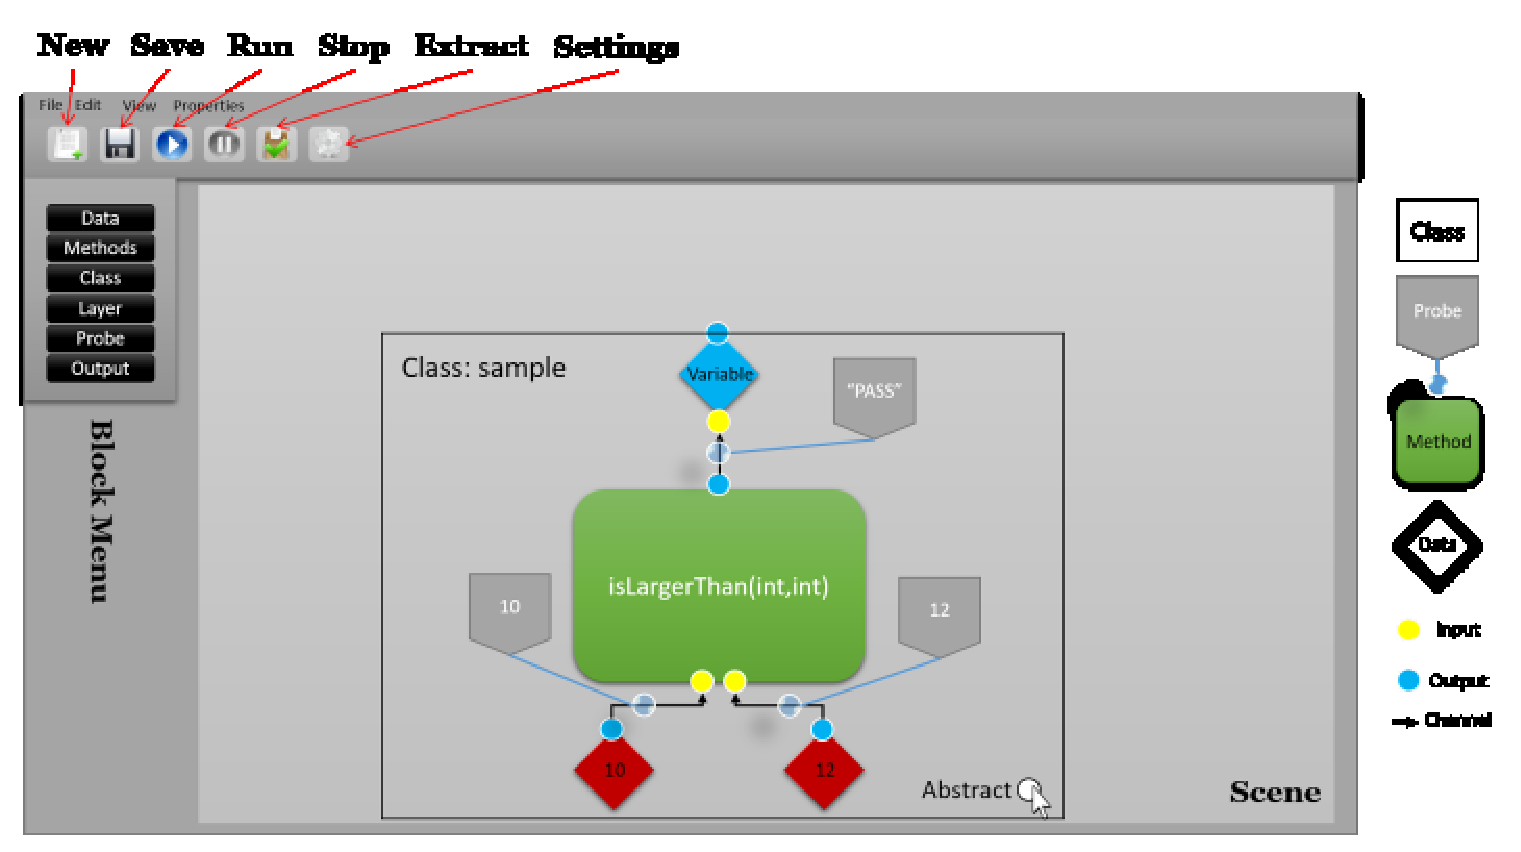
\includegraphics[width=0.5\textwidth]{graphics/mocksize.eps}}\\
		\label{fig:fig1}
		\caption{A proposed layout of the menu and build space.}
	\end{minipage}
	\end{figure}
	\noindent \textbf{Performance Metrics}\\
	\indent We desire to create a graphical user interface that translates user input into executable code. 
	Our software must follow a simple flowchart design where each node and line drawn represents a line of code that compiles and outputs relevant data.
	For our software to be successful it must create an executable Python file in the background that can be extracted at the push of a button. 
	To measure whether our solution's debugging functionality works properly we will observe how well it communicates errors to the user through alerts.
	 Running a suite of tests will allow us to ensure that the interface catches and displays errors to the user and provides advice as to how to fix the errors.
	 Our software needs to be easy to understand.
	 By hosting weekly trials of our software with volunteers we will gather data through questionnaires on what workspace layouts provide a more comfortable experience for users.
	 
	 
	 
\end{document}
